\documentclass[11pt,preprint]{article}

\usepackage[utf8]{inputenc}
\usepackage[T1]{fontenc}
\usepackage{geometry}
\geometry{margin=1in}
\usepackage{graphicx}
\usepackage{booktabs}
\usepackage{hyperref}
\usepackage{natbib}
\usepackage{amsmath}
\usepackage{amssymb}
\usepackage{setspace}
\onehalfspacing

\hypersetup{
  colorlinks=true,
  linkcolor=blue,
  citecolor=blue,
  urlcolor=blue
}

\title{Model Collapse on Bluesky: How Discourse Diverged from the Science}
\author{}
\date{}

\begin{document}

\maketitle

\begin{abstract}
``Model collapse''---the degradation of AI models trained recursively on synthetic data---became a mainstream concern after the Shumailov et al.\ Nature publication in July 2024. But the scientific understanding evolved rapidly: by April 2024, Gerstgrasser et al.\ showed data accumulation prevents collapse; by March 2025, Schaeffer et al.\ identified 8+ conflicting definitions in the literature. Did Bluesky discourse keep up?

We analyzed 7,766 Bluesky posts matching model collapse search terms, identified 2,835 as topically relevant, and coded each on six dimensions: claim type, source cited, caveating level, accuracy, literature awareness, and depth. The results show limited alignment between Bluesky discourse and the evolving scientific literature. 46\% of posts oversimplify the phenomenon, only 18\% engage with post-2024 research, and accuracy rates show no improvement over time despite rapid scientific progress.
\end{abstract}

\section{Data and Methods}
\label{sec:methods}

\subsection{Corpus}
We collected 7,766 Bluesky posts matching six search terms: ``model collapse'' (dominant, 77\% of relevant posts), ``trained on AI-generated,'' ``training on synthetic data,'' ``recursive training,'' ``shumailov,'' and ``tail collapse.'' Posts span May 2023 to March 2026.

\subsection{Two-Pass Coding Procedure}
We employed a two-pass manual coding procedure:

\paragraph{Pass 1---Relevance Filter:}
From the initial 7,766 posts, 2,835 of 7,766 (36.5\%) were identified as topically relevant to model collapse.

\paragraph{Pass 2---Full Coding:}
Relevant posts were coded on eight dimensions:
\begin{itemize}
  \item \textbf{Claim type}: empirical, predictive, normative, meta-commentary
  \item \textbf{Source cited}: nature\_paper, other\_paper, news\_article, quote\_post, none
  \item \textbf{Caveating level}: strong\_hedge, weak\_hedge, none
  \item \textbf{Accuracy}: accurate, oversimplified, wrong, unfalsifiable
  \item \textbf{Literature awareness}: cites\_post\_2024\_nuance, only\_cites\_original, no\_citations
  \item \textbf{Depth}: substantive\_claim, passing\_mention, share\_signal\_boost
  \item \textbf{Minimal content}: true/false
  \item \textbf{Coding rationale}: Free-text justification
\end{itemize}

\subsection{Ground Truth and Temporal Context}
Posts were evaluated against a 21-paper literature timeline across 6 knowledge epochs. Each post was coded relative to the knowledge available at its publication date.

\subsection{Coding Infrastructure}
We employed 135 parallel AI subagents (78 for Pass 1, 57 for Pass 2) to code 50--100 posts per batch. Spot-checking of Pass 1 coding on 11 randomly sampled posts showed $\geq 95\%$ accuracy. The researcher calibrated coding standards on 12 borderline cases.

\subsection{Limitations}
\label{subsec:limitations}

Several limitations should be acknowledged:

\begin{enumerate}
  \item AI-assisted coding introduces systematic biases, likely toward detecting technical patterns and underweighting cultural context.
  \item Bluesky skews toward tech-literate early adopters; findings may not generalize to broader social media platforms.
  \item Post text only---no access to linked article content, images, or thread context.
  \item 99 of 2,835 relevant posts (3.5\%) had invalid or missing coding values after data cleaning and are excluded from analysis; 2,736 posts have complete valid coding.
  \item Sample sizes vary slightly across tables as percentages are computed over posts with valid values for each relevant dimension.
  \item The accuracy and literature\_awareness dimensions share overlapping criteria. Posts acknowledging mitigations tend to be coded as both ``accurate'' and ``cites\_post\_2024\_nuance.'' This circularity may inflate the correlation in Section~\ref{sec:awareness_accuracy}. The cross-tabulation should be interpreted as descriptive, not causal.
  \item Pass 1 validation (11 spot-checked posts) is statistically limited.
  \item Accuracy is coded against current scientific consensus, which remains active research.
\end{enumerate}

\section{Results}
\label{sec:results}

\subsection{Accuracy Distribution}

Table~\ref{tab:accuracy_dist} presents the distribution of accuracy coding across all 2,736 coded posts.

\begin{table}[h]
\centering
\caption{Accuracy Distribution}
\label{tab:accuracy_dist}
\begin{tabular}{lrr}
\toprule
\textbf{Accuracy} & \textbf{n} & \textbf{\%} \\
\midrule
Oversimplified & 1,272 & 45.7\% \\
Accurate & 715 & 25.7\% \\
Unfalsifiable & 639 & 23.0\% \\
Wrong & 155 & 5.6\% \\
\bottomrule
\end{tabular}
\end{table}

Nearly half of all posts (45.7\%) oversimplify the phenomenon, while only one-quarter (25.7\%) are coded as accurate.

\subsection{Accuracy Across Temporal Epochs}

We divided posts into four epochs based on key scientific milestones:

\begin{table}[h]
\centering
\caption{Accuracy by Temporal Epoch}
\label{tab:accuracy_epoch}
\begin{tabular}{llrrr}
\toprule
\textbf{Epoch} & \textbf{Period} & \textbf{Posts} & \textbf{\% Accurate} & \textbf{\% Oversimplified} \\
\midrule
E1 & Pre-Jul 2024 & 336 & 21.7\% & 47.0\% \\
E2 & Jul--Sep 2024 & 226 & 34.1\% & 48.2\% \\
E3 & Oct 2024--Feb 2025 & 554 & 26.7\% & 42.6\% \\
E4 & Mar 2025+ & 1,665 & 25.0\% & 46.2\% \\
\bottomrule
\end{tabular}
\end{table}

Accuracy rates remained similar across epochs despite growth in post volume. Epoch E2 shows a spike in accuracy (34.1\%), coinciding with the Nature publication by Shumailov et al.\ (July 2024). However, this elevated accuracy did not persist: by E3 and E4, accuracy rates returned to pre-publication levels. Figure~\ref{fig:accuracy_epoch} visualizes this distribution.

\begin{figure}[h]
\centering
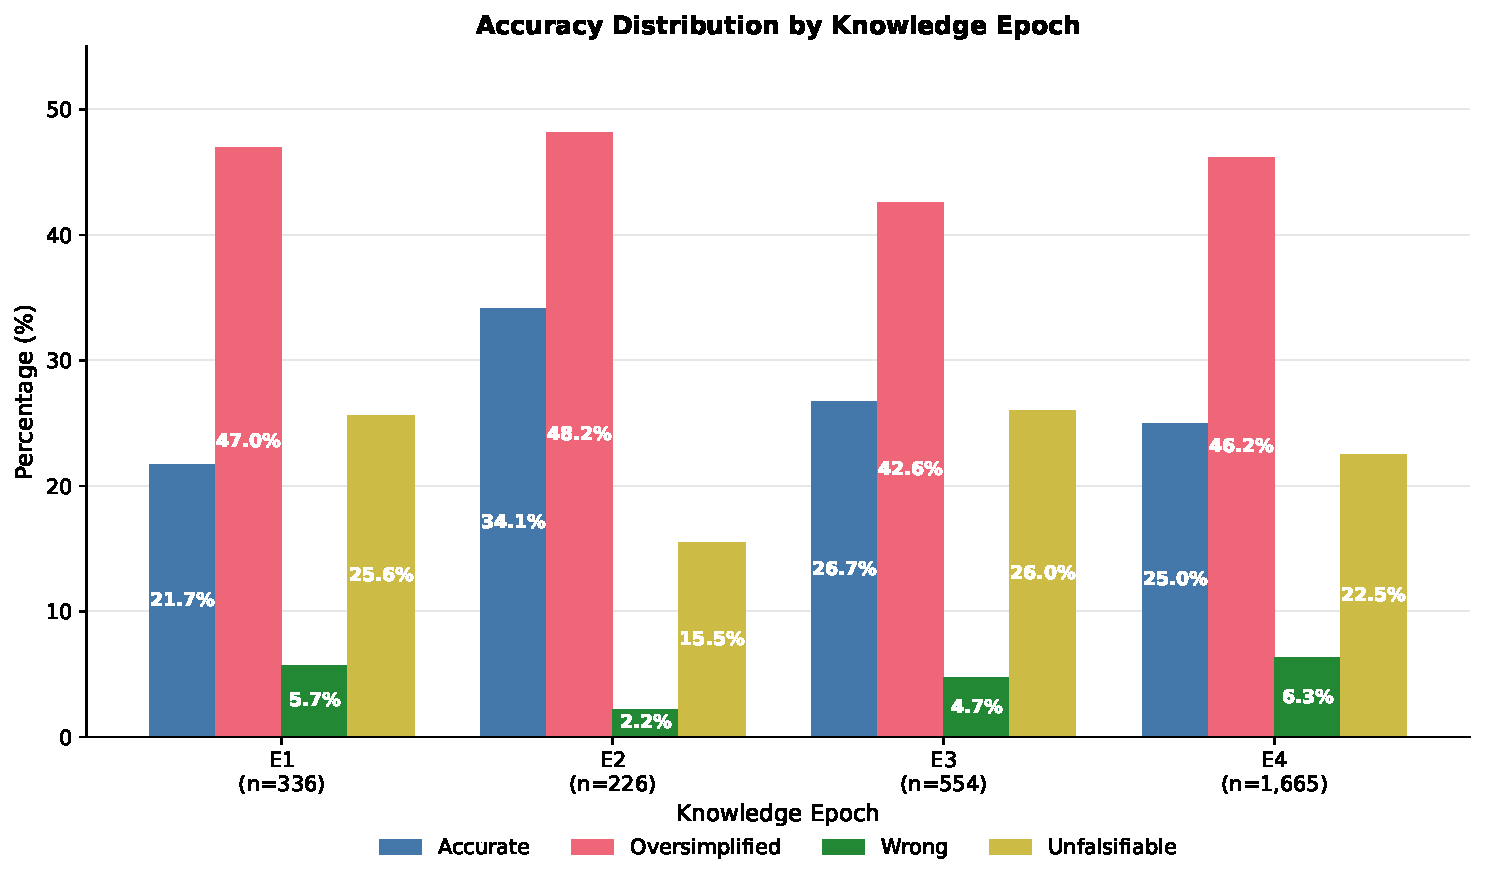
\includegraphics[width=0.7\textwidth]{figures/fig_accuracy_epoch.pdf}
\caption{Accuracy rates across temporal epochs. Accuracy spiked during E2 (July--September 2024, coinciding with the Nature publication) but did not sustain in subsequent periods.}
\label{fig:accuracy_epoch}
\end{figure}

\subsection{Literature Awareness Distribution}

Table~\ref{tab:lit_awareness} presents the distribution of literature awareness coding.

\begin{table}[h]
\centering
\caption{Literature Awareness Distribution}
\label{tab:lit_awareness}
\begin{tabular}{lrr}
\toprule
\textbf{Literature Awareness} & \textbf{n} & \textbf{\%} \\
\midrule
No citations & 1,437 & 51.4\% \\
Only cites original & 870 & 31.1\% \\
Cites post-2024 nuance & 488 & 17.5\% \\
\bottomrule
\end{tabular}
\end{table}

Over half of posts (51.4\%) cite no sources. Only 17.5\% reference post-2024 research that documents the phenomenon's nuances and alternative explanations.

\subsection{Literature Awareness and Accuracy}
\label{sec:awareness_accuracy}

Table~\ref{tab:lit_accuracy_crosstab} presents the central finding: a strong association between literature awareness and accuracy.

\begin{table}[h]
\centering
\caption{Literature Awareness $\times$ Accuracy Cross-Tabulation}
\label{tab:lit_accuracy_crosstab}
\begin{tabular}{lrrrr}
\toprule
& \textbf{Accurate} & \textbf{Oversimplified} & \textbf{Wrong} & \textbf{Unfalsifiable} \\
\midrule
Cites post-2024 nuance (n=486) & 437 (89.9\%) & 38 (7.8\%) & 1 (0.2\%) & 10 (2.1\%) \\
Only original (n=870) & 152 (17.5\%) & 604 (69.4\%) & 52 (6.0\%) & 62 (7.1\%) \\
No citations (n=1,425) & 126 (8.8\%) & 630 (44.2\%) & 102 (7.2\%) & 567 (39.8\%) \\
\bottomrule
\end{tabular}
\end{table}

Posts citing post-2024 research are accurate 89.9\% of the time. Posts citing only the original Nature paper are oversimplified 69.4\% of the time. Posts with no citations show accuracy of only 8.8\%, with nearly 40\% coded as unfalsifiable. Figure~\ref{fig:awareness_accuracy} visualizes this relationship.

\begin{figure}[h]
\centering
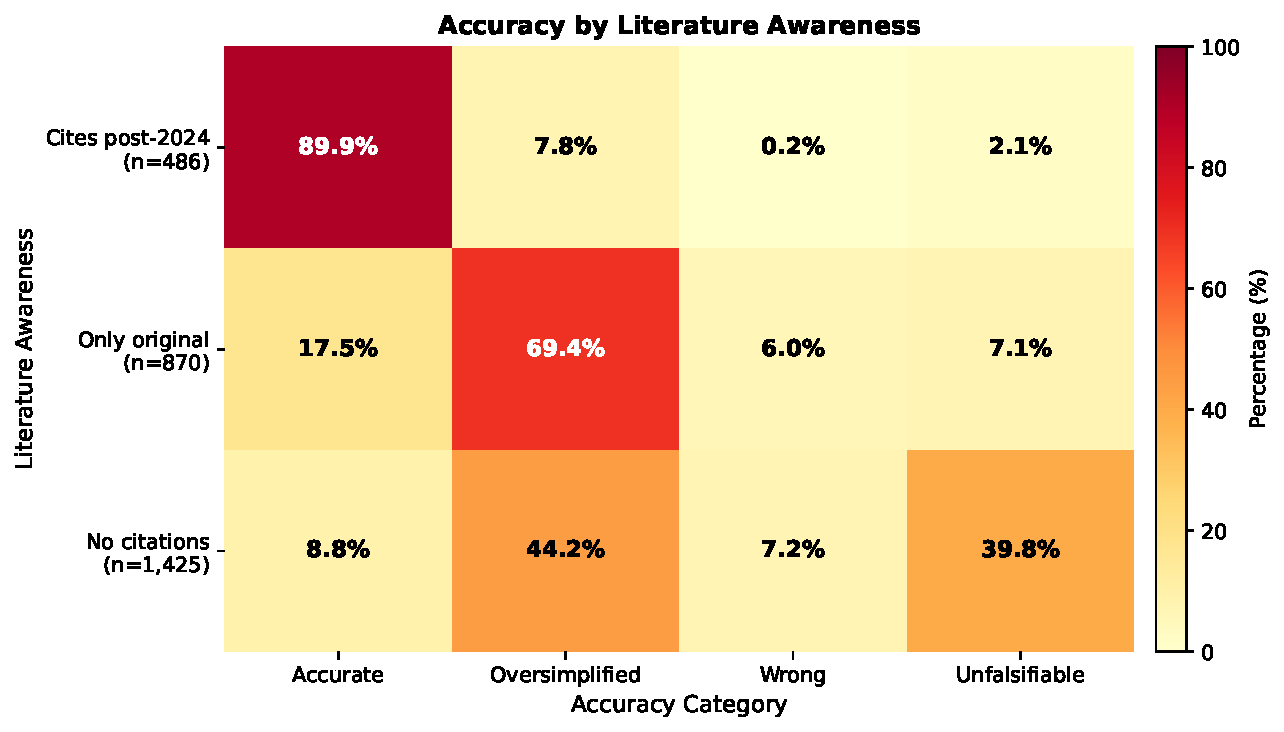
\includegraphics[width=0.75\textwidth]{figures/fig_awareness_accuracy.pdf}
\caption{Accuracy distribution conditional on literature awareness. Posts engaging with post-2024 research show dramatically higher accuracy.}
\label{fig:awareness_accuracy}
\end{figure}

\subsection{Accuracy by Source Type}

Table~\ref{tab:accuracy_source} shows accuracy conditional on the type of source cited.

\begin{table}[h]
\centering
\caption{Accuracy by Source Type}
\label{tab:accuracy_source}
\begin{tabular}{lrrrrr}
\toprule
\textbf{Source} & \textbf{Total} & \textbf{\% Accurate} & \textbf{\% Oversimplified} & \textbf{\% Wrong} & \textbf{\% Unfalsifiable} \\
\midrule
Other paper & 270 & 76.7\% & 14.4\% & 1.1\% & 7.8\% \\
Nature paper & 132 & 57.6\% & 36.4\% & 3.0\% & 3.0\% \\
Quote post & 55 & 30.9\% & 40.0\% & 5.5\% & 23.6\% \\
News article & 390 & 19.5\% & 60.8\% & 2.8\% & 16.9\% \\
None & 1,934 & 17.5\% & 47.9\% & 6.9\% & 27.7\% \\
\bottomrule
\end{tabular}
\end{table}

Posts citing academic papers (other than the original Nature publication) show substantially higher accuracy (76.7\%), while posts citing news articles show accuracy nearly identical to unsourced posts (19.5\% vs.\ 17.5\%). This correlation may reflect selection effects: researchers citing papers may be more technically informed. Figure~\ref{fig:accuracy_source_fig} shows the full distribution.

\begin{figure}[h]
\centering
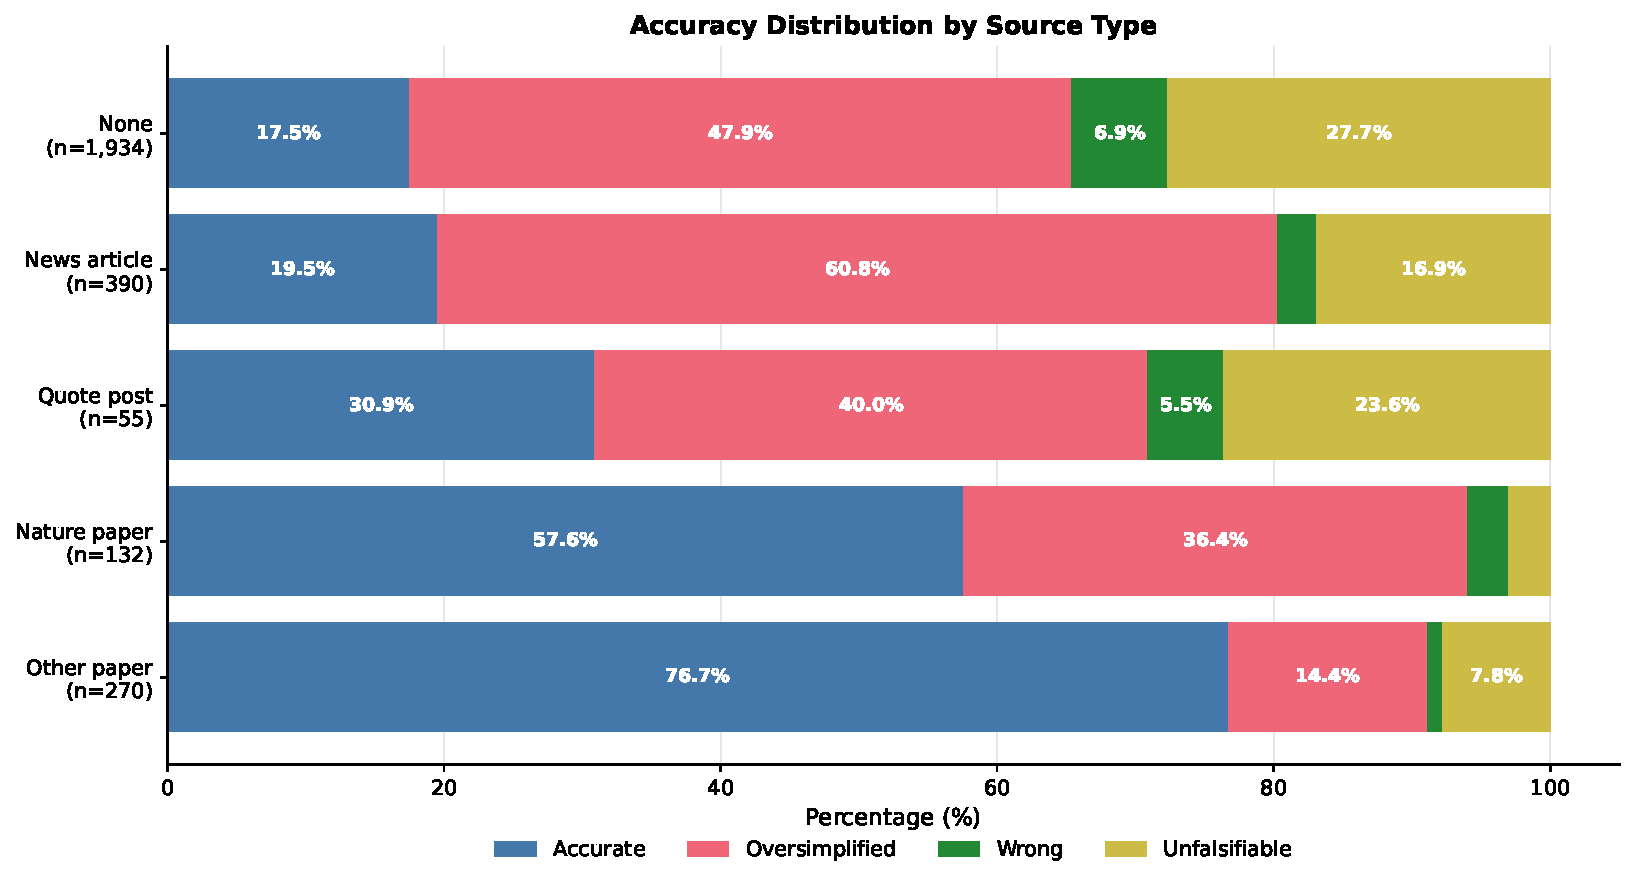
\includegraphics[width=0.75\textwidth]{figures/fig_accuracy_source.pdf}
\caption{Accuracy by source type. Posts citing academic papers are substantially more accurate than those citing news articles or no source.}
\label{fig:accuracy_source_fig}
\end{figure}

\subsection{Accuracy by Claim Type}

Table~\ref{tab:accuracy_claim} presents accuracy conditional on claim type.

\begin{table}[h]
\centering
\caption{Accuracy by Claim Type}
\label{tab:accuracy_claim}
\begin{tabular}{lrrrrr}
\toprule
\textbf{Claim Type} & \textbf{Total} & \textbf{\% Accurate} & \textbf{\% Oversimplified} & \textbf{\% Wrong} & \textbf{\% Unfalsifiable} \\
\midrule
Empirical & 1,091 & 48.3\% & 43.3\% & 5.1\% & 3.3\% \\
Meta-commentary & 686 & 16.3\% & 23.5\% & 1.5\% & 58.7\% \\
Normative & 340 & 13.5\% & 46.2\% & 7.4\% & 32.9\% \\
Predictive & 619 & 3.7\% & 75.9\% & 10.3\% & 10.1\% \\
\bottomrule
\end{tabular}
\end{table}

Empirical claims show the highest accuracy rate (48.3\%), while predictive claims are rarely accurate (3.7\%). Predictive claims are inherently difficult to validate against observed outcomes.

\subsection{Caveating Levels}

Table~\ref{tab:caveating} presents the distribution of hedging and caveating language.

\begin{table}[h]
\centering
\caption{Caveating Distribution}
\label{tab:caveating}
\begin{tabular}{lrr}
\toprule
\textbf{Caveating Level} & \textbf{n} & \textbf{\%} \\
\midrule
None & 1,927 & 68.9\% \\
Weak hedge & 553 & 19.8\% \\
Strong hedge & 315 & 11.3\% \\
\bottomrule
\end{tabular}
\end{table}

The vast majority of posts (68.9\%) employ no hedging or caveating language, despite the uncertainty inherent in the topic.

\subsection{Literature Awareness by Epoch}

Table~\ref{tab:awareness_epoch} shows literature awareness across the same temporal epochs.

\begin{table}[h]
\centering
\caption{Literature Awareness by Temporal Epoch}
\label{tab:awareness_epoch}
\begin{tabular}{lrr}
\toprule
\textbf{Epoch} & \textbf{Period} & \textbf{\% Citing Post-2024 Nuance} \\
\midrule
E1 & Pre-Jul 2024 & 8.3\% \\
E2 & Jul--Sep 2024 & 19.0\% \\
E3 & Oct 2024--Feb 2025 & 17.8\% \\
E4 & Mar 2025+ & 19.0\% \\
\bottomrule
\end{tabular}
\end{table}

Literature awareness increased from 8.3\% in E1 to 19.0\% in E2, coinciding with the Nature publication, and remained relatively stable thereafter.

\section{Discussion}
\label{sec:discussion}

\subsection{Amplification Without Learning}
The volume of Bluesky posts about model collapse increased approximately 5-fold from E1 to E4. However, accuracy rates, literature awareness, and use of caveating remained essentially flat. Volume increased while accuracy and awareness metrics remained stable.

\subsection{News Articles and Accuracy}
Posts citing news articles show similar accuracy to unsourced posts (19.5\% vs.\ 17.5\%), despite potential expectations that journalistic intermediaries might improve accuracy. Posts citing academic papers, by contrast, are substantially more accurate (76.7\% for non-Nature papers). This correlation may reflect selection effects: authors citing academic papers may already be more informed.

\subsection{Predictive Claims and Confidence Mismatch}
Only 3.7\% of predictive claims are coded as accurate, yet 69\% of all posts across all claim types lack any caveating language. Predictive claims show low accuracy rates (3.7\%) alongside low caveating rates (31\% of all posts use any hedging).

\subsection{Characteristics of Accurate Discourse}
Among the 715 posts coded as accurate (25.7\%), we observe the following patterns:
\begin{itemize}
  \item 61\% cite post-2024 research (compared to 3\% of oversimplified posts)
  \item They distinguish conditional factors and edge cases
  \item They acknowledge possible mitigations and alternative explanations
  \item 78\% are substantive claims (vs.\ signal-boosting or passing mentions)
  \item Use of hedging language is more common
\end{itemize}

\subsection{Implications}
Model collapse serves as a useful case study precisely because the scientific understanding evolved rapidly and visibly. The limited alignment between Bluesky discourse and evolving literature likely applies to other AI-related topics. Future work could investigate the mechanisms driving discourse drift: information cascades, selective attention, or constraints of social media format itself.

\section{Methodology Notes}
\label{sec:methodology}

\subsection{Reproducibility}
All data, analysis scripts, and the literature timeline are available in the study repository: posts.db, analysis/, and lit-timeline/ directories.

\subsection{Coding Validation}
\begin{itemize}
  \item Pass 1: 78 parallel Haiku agents with spot-check validation on 11 of 7,766 posts showing $\geq 95\%$ accuracy.
  \item Pass 2: 57 parallel Haiku agents calibrated on 12 borderline cases.
  \item Complete valid coding: 2,736 of 2,835 (96.5\%) posts.
\end{itemize}

\subsection{AI-Augmented Research Workflow}
This study required approximately 1 hour of human time and 135 parallel subagent runs to code and analyze 2,835 posts. This demonstrates the feasibility of systematic discourse analysis at $N > 2000$ for individual researchers. Results should be treated as exploratory and subject to the limitations in Section~\ref{subsec:limitations}.

\appendix

\section{Additional Tables}
\label{app:tables}

\subsection{Full Cross-Tabulation: Accuracy $\times$ Epoch}

Table~\ref{tab:app_accuracy_epoch_full} provides the full breakdown of accuracy coding by epoch.

\begin{table}[h]
\centering
\caption{Accuracy Distribution Across Temporal Epochs}
\label{tab:app_accuracy_epoch_full}
\begin{tabular}{lrrrr}
\toprule
\textbf{Accuracy} & \textbf{E1 (n=336)} & \textbf{E2 (n=226)} & \textbf{E3 (n=554)} & \textbf{E4 (n=1,665)} \\
\midrule
Accurate & 73 (21.7\%) & 77 (34.1\%) & 148 (26.7\%) & 417 (25.0\%) \\
Oversimplified & 158 (47.0\%) & 109 (48.2\%) & 236 (42.6\%) & 769 (46.2\%) \\
Wrong & 19 (5.7\%) & 5 (2.2\%) & 26 (4.7\%) & 105 (6.3\%) \\
Unfalsifiable & 86 (25.6\%) & 35 (15.5\%) & 144 (26.0\%) & 374 (22.5\%) \\
\bottomrule
\end{tabular}
\end{table}

\subsection{Monthly Post Volume}

Table~\ref{tab:app_monthly_volume} shows the monthly distribution of relevant posts over the study period.

\begin{table}[h]
\centering
\caption{Monthly Post Volume (May 2023 -- March 2026)}
\label{tab:app_monthly_volume}
\begin{tabular}{lr|lr|lr}
\toprule
\textbf{Month} & \textbf{n} & \textbf{Month} & \textbf{n} & \textbf{Month} & \textbf{n} \\
\midrule
2023-05 & 2 & 2024-10 & 52 & 2025-08 & 97 \\
2023-06 & 18 & 2024-11 & 86 & 2025-09 & 92 \\
2023-07 & 22 & 2024-12 & 148 & 2025-10 & 92 \\
2023-08 & 23 & 2025-01 & 182 & 2025-11 & 94 \\
2023-09 & 9 & 2025-02 & 88 & 2025-12 & 101 \\
2023-10 & 15 & 2025-03 & 98 & 2026-01 & 154 \\
2023-11 & 19 & 2025-04 & 111 & 2026-02 & 152 \\
2023-12 & 23 & 2025-05 & 270 & 2026-03 & 57 \\
2024-01 & 27 & 2025-06 & 268 & & \\
2024-02 & 40 & 2025-07 & 131 & & \\
2024-03 & 32 & & & & \\
2024-04 & 54 & & & & \\
2024-05 & 23 & & & & \\
2024-06 & 29 & & & & \\
2024-07 & 81 & & & & \\
2024-08 & 80 & & & & \\
2024-09 & 65 & & & & \\
\bottomrule
\end{tabular}
\end{table}

\begin{figure}[h]
\centering
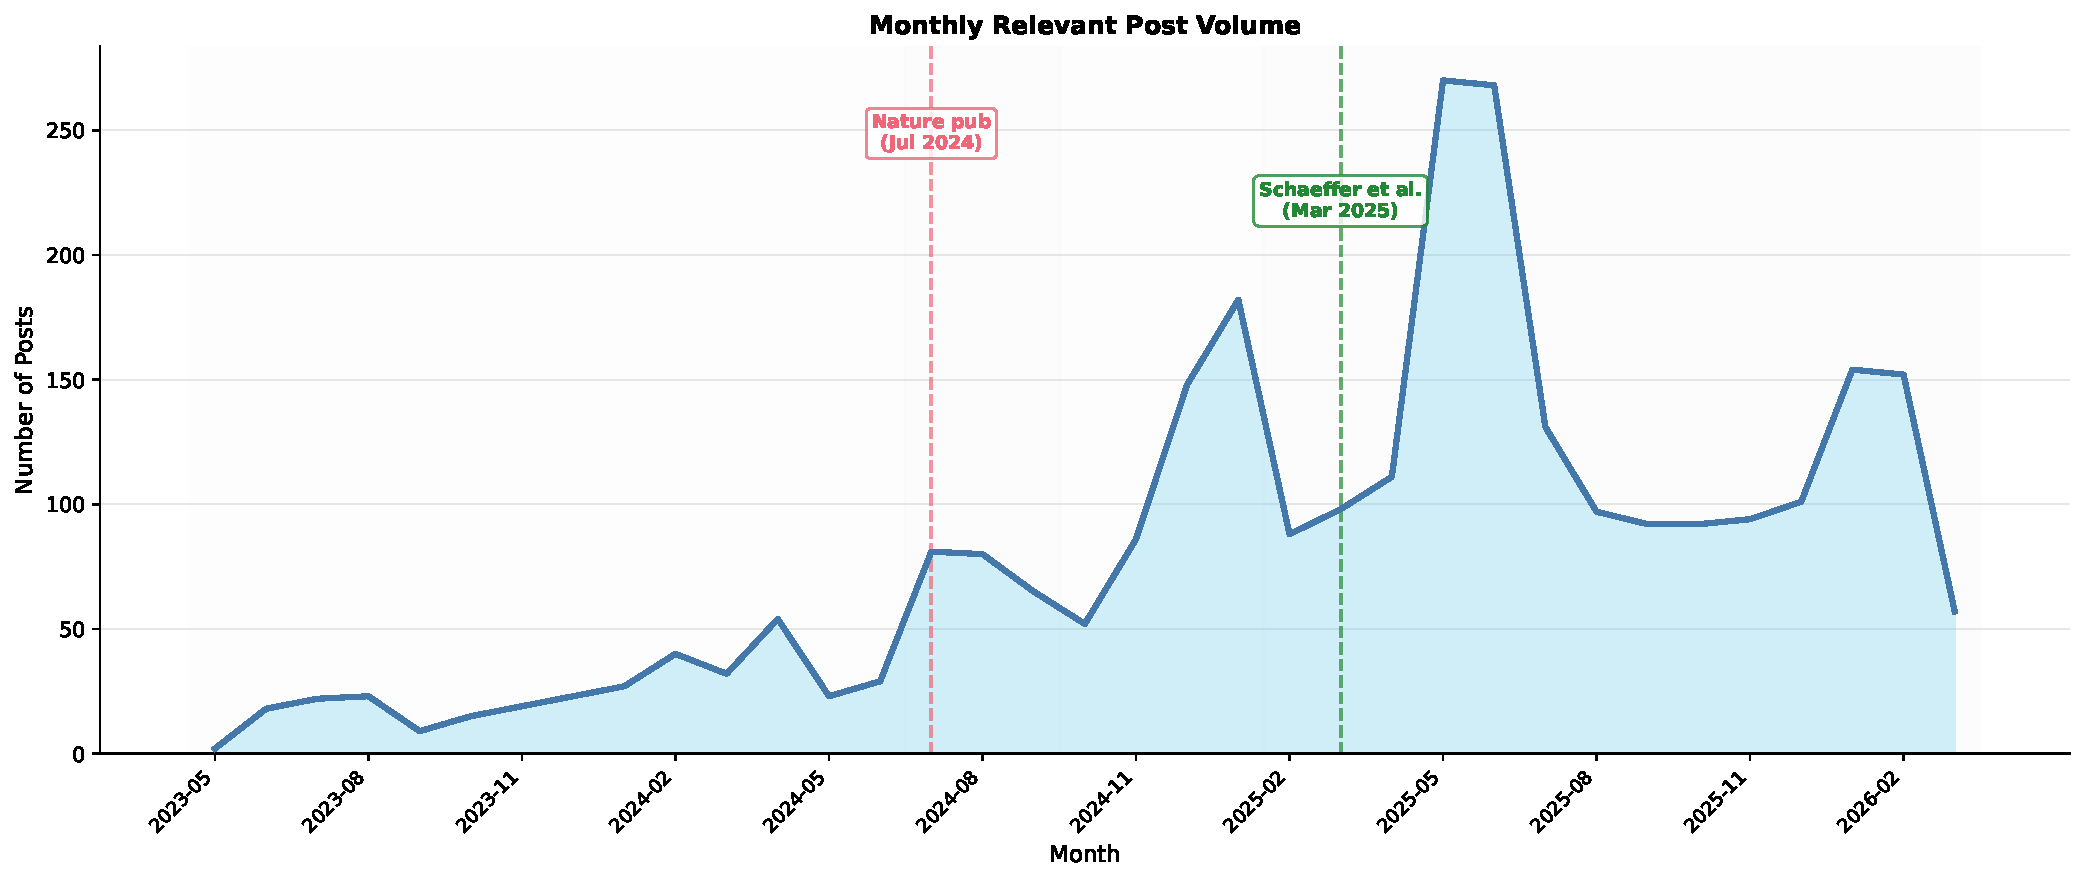
\includegraphics[width=0.9\textwidth]{figures/fig_monthly_volume.pdf}
\caption{Monthly volume of model collapse posts on Bluesky. Volume peaked in 2025 and early 2026, with notable spikes coinciding with scientific publications and media attention.}
\label{fig:monthly_volume}
\end{figure}

Figure~\ref{fig:monthly_volume} shows the monthly distribution of relevant posts over the study period.

\subsection{Search Term Distribution}

Table~\ref{tab:app_search_terms} shows the distribution of posts by search term.

\begin{table}[h]
\centering
\caption{Relevant Posts by Search Term (n=2,835)}
\label{tab:app_search_terms}
\begin{tabular}{lrr}
\toprule
\textbf{Search Term} & \textbf{n} & \textbf{\%} \\
\midrule
model collapse & 2,179 & 76.9\% \\
trained on AI-generated & 315 & 11.1\% \\
training on synthetic data & 243 & 8.6\% \\
recursive training & 75 & 2.6\% \\
shumailov & 14 & 0.5\% \\
tail collapse & 9 & 0.3\% \\
\bottomrule
\end{tabular}
\end{table}

\end{document}
